\section{Experimental Setup and Measurements}
\label{sec:procedure}
\begin{figure}
    \centering
    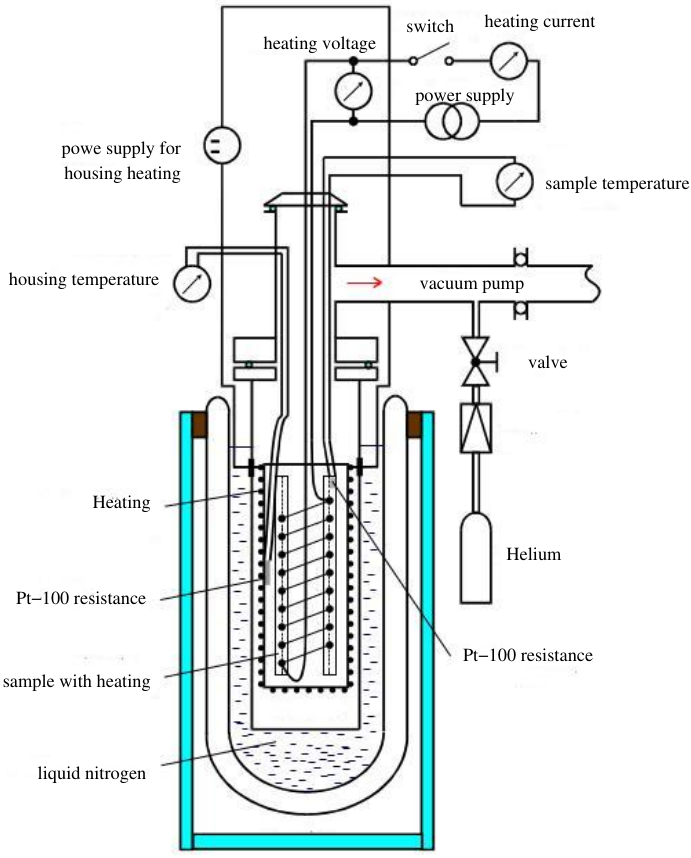
\includegraphics[width=\textwidth]{pictures/setup.png}
    \caption{Schematic illustration of the experimental setup. \cite{V47}}
    \label{fig:setup}
\end{figure}

The experimental setup consists of a cryogenic storage dewar, a type of vacuum flask. 
Inside this dewar, there is a recipient filled with \SI{342}{\gram} of copper. 
Both the probe and the vessel are heated using an electric heating coil. 
This setup is schematically illustrated in Figure \ref{fig:setup}.

Initially, the recipient is evacuated. 
Subsequently, the dewar is filled with liquid nitrogen to cool the probe 
down to \SI{80}{\kelvin}. 
To ensure effective thermal conduction during the cooling process, 
the recipient is filled with helium. 
The temperature $T$ is not measured directly but inferred from the resistance $R$. 
The temperature can be calculated using the equation
\begin{equation}
    T=\num{0.00134}R^2+\num{2.296}R-243.02
    \label{eqn:rzut}
\end{equation}
where the resistance $R$ is measured in \si{\ohm}, and the temperature is 
calculated in \si{\celsius}.
A temperature of \SI{80}{\kelvin} corresponds to a resistance of approximately 
\SI{22}{\ohm}. 

After cooling, the recipient is evacuated again. 
The heating coil is set to a constant current of \SI{150}{\milli\ampere}, 
resulting in an increase in resistance.
A second coil ensures that the temperatures of the probe and 
the vessel remain equal. 

The current and the resistance of both coils are measured every \SI{2}{\minute}.
The measurement concludes once the temperature reaches \SI{300}{\kelvin}.
